\documentclass[a4paper]{article}

\usepackage[T1]{fontenc}
\usepackage[utf8]{inputenc}
\usepackage[french]{babel}
\usepackage{mathpazo}
\usepackage[scaled]{helvet}
\usepackage{courier}
\usepackage[margin=20mm]{geometry}
\usepackage{tabularx}
\usepackage{graphicx}


\makeatletter
\newenvironment{expl}{%
  \begin{list}{}{%
      \small\itshape%
      \topsep\z@%
      \listparindent0pt%\parindent%
      \parsep0.75\baselineskip%\parskip%
      \setlength{\leftmargin}{20mm}%
      \setlength{\rightmargin}{20mm}%
    }
  \item[]}%
  {\end{list}}
\makeatother

\title{Rapport du Projet  \\ Intelligence Artificielle }
\author{Abdelheq DELMI BOURAS \\ Siham JANATI }
\date{Mars 2021}

\begin{document}

\maketitle

% Mettez une table des matières si votre rapport contient plus
% de 3 pages ou si vous ne suivez pas le plan suggéré :
%\tableofcontents

% supprimez toutes les explications comprises entre \begin{expl}
% et \end{expl} dans votre rapport.




\section{Préparation des données:}

\subsection{Recensement des données }\label{sec-shm}

\begin{expl}
\begin{center}
   \begin{tabular}{ l | c || r | }
     \hline
     0 (inlier) & 250  \\ \hline
     1 (outlier) &80  \\ \hline
     \hline
   \end{tabular}
 \end{center}


\end{expl}

% \subsection{Autres données partagées}
% 
% \begin{expl}
%   Indiquez toutes les autres données partagées entre certains ou tous
%   les processus. La forme est la même que dans la section précédente.
%   Précisez aussi à quel moment ces données sont créées, et à quel
%   moment elles disparaissent.
% \end{expl}

\subsection{Visualisation des données}
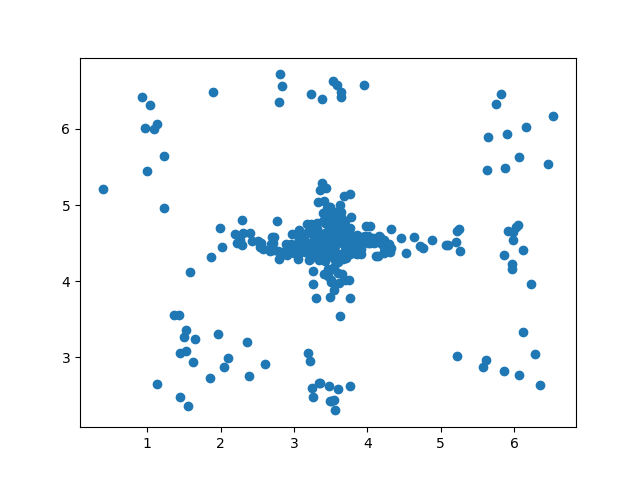
\includegraphics[width=\textwidth]{Figure_1.png}

\subsection{description des données:}
\begin{expl}
    dans la figure présentée ci-dessus, on aperçoit de manière approximative,  que les inliers se présentent dans la section  x[1,7:5,2]  et y[3,4:5,2]
\end{expl}

\section{SIHAM PARTIE 2}

\begin{expl}
  Chacune des sous-sections suivantes doit décrire un aspect de la
  synchronisation. Elles ont toutes la même organisation, et doivent
  contenir deux ou trois parties clairement délimitées.

  La première partie décrit tous les objets impliqués dans la
  synchronisation de l'accueil des groupes dans le restaurant. Il
  s'agit des données «~normales~» (par exemple un entier) et des
  sémaphores. Pour chacun de ces éléments, précisez si il est rattaché
  au restaurant globalement ou à un groupe (ou encore à un convive).

  Par exemple, si le restaurant était muni au bar de distributeurs de
  gel hydroalcoolique grâce auxquels les convives peuvent se nettoyer les
  mains, il faudrait mentionner~:

  \begin{tabularx}{\linewidth}{|l|l|X|}
    \hline
    distributeurs & sem\_t & le sémaphore représentant le nombre de
    distributeurs \underline{du restaurant} (voir section~\ref{sec-shm})
    \\ \hline
    monid & int & le nom \underline{du convive}
    \\ \hline
  \end{tabularx}

  La seconde partie doit contenir un pseudo-code de ce qu'exécute
  \emph{chaque} acteur impliqué (le restaurant, le convive, autres).
  Seuls les aspects importants doivent être présentés~: opérations sur
  les sémaphores, affectation de valeurs aux variables
  partagées... Le reste (par exemple les messages liés à
  \texttt{DEBUG\_OUTPUT}) ne doivent pas apparaître ici.

  Dans l'exemple des distributeurs de gel, le pseudo-code serait~:

\begin{verbatim}
// Ce code est exécuté par le convive
P (distributeurs)
se_laver_les_mains (monid)
V (distributeurs)
\end{verbatim}

  La troisième partie contient toutes les remarques que vous jugerez
  pertinentes. Vous pouvez par exemple y préciser les conditions de
  concurrence, ou les éventuelles limitations ou propriétés
  remarquables de votre solution.

  Dans l'exemple des distributeurs de gel, vous pourriez préciser que
  vous avez pensé à implémenter à la place une attente limitée dans le
  temps pour les convives qui portaient des gants en entrant (en
  expliquant comment vous auriez fait), mais que cela aurait compliqué
  le code pour un intérêt limité.

  Vous pouvez ajouter des sous-sections si vous avez d'autres
  synchronisations importantes, ou fragmenter celles qui vous sont
  proposée ci-dessous.
\end{expl}


\subsection{Arrivée d'un convive}

\begin{expl}
  Expliquez dans cette sous-section, conformément aux indications
  ci-dessus, tout ce qui se passe lorsqu'un convive arrive au
  restaurant, ainsi que toutes les informations échangées pendant
  cette prise en charge. N'oubliez pas d'indiquer qui (restaurant~?
  convive~? autre~?) exécute quel code.
\end{expl}

\subsection{Contrôle des autorités}

\begin{expl}
  Cette section explique en détail tout ce qui se passe lors d'un
  contrôle des autorités. Donnez le détail du mécanisme de
  transmission du cahier de rappels.
\end{expl}

\subsection{Ouverture et fermeture du restaurant}

\begin{expl}
  Expliquez l'effet de l'ouverture et de la fermeture du restaurant
  sur tous les processus actifs (vous pouvez faire deux sections
  distinctes si vous le jugez utile). Précisez clairement quel code
  est exécuté par qui, et ne répétez pas du code déjà donné plus haut.
\end{expl}

\section{Remarques sur l'implémentation}

\begin{expl}
  Placez ici toute remarque relative à vos choix d'implémentation (si
  vous en avez). Par exemple~: si vous avez placé des temporisations
  particulières pour vérifier que certains cas de concurrence étaient
  gérés correctement, expliquez cela dans cette section. Toute autre
  remarque qui aide à comprendre votre code est à placer ici.
\end{expl}

\section{Conclusion}

\begin{expl}
  Tirez les conclusions de votre projet~: limites de votre
  implémentation, difficultés particulières, subtilités dont vous êtes
  fiers, etc.
\end{expl}

\end{document}
